\documentclass[12pt]{article}
    \usepackage{times}
    \usepackage[latin1]{inputenc}
    \usepackage[frenchb]{babel}
    \usepackage{graphicx}
    \usepackage[numbers]{natbib}
    \usepackage{amsfonts}
    \usepackage{amsmath}

    \numberwithin{equation}{section}
    \numberwithin{figure}{section}
    \numberwithin{table}{section}

    \usepackage[nooneline]{subfigure}
    \usepackage{bm}
%    \usepackage{prelim2e}
    \usepackage{booktabs}
    \usepackage{color}
    \usepackage{rotating}
    \usepackage{afterpage}
%    \usepackage[draft]{fixme}
    \usepackage{refstyle}
        \newref{equ}{refcmd=(\ref{#1}),name=�quation~,Name=�quation~,names=�quations~,Names=�quation~,lsttxt={\ et\ },rngtxt={\ �\ }}
        \newref{fig}{name=figure~,names=figures~,Name=Figure~,Names=Figures~,lsttxt={\ et\ },rngtxt={\ �\ }}
        \newref{subfig}{name=figure~,names=figures~,Name=Figure~,Names=Figures~,lsttxt={\ et\ },rngtxt={\ �\ }}
        \newref{chap}{name=chapitre~,names=chapitres~,Name=Chapitre~,Names=Chapitres~,lsttxt={\ et\ },rngtxt={\ �\ }}
        \newref{sect}{name=section~,names=sections~,Name=Section~,Names=Sections~,lsttxt={\ et\ },rngtxt={\ �\ }}
        \newref{ssect}{name=section~,names=sections~,Name=Section~,Names=Sections~,lsttxt={\ et\ },rngtxt={\ �\ }}
        \newref{sssect}{name=section~,names=sections~,Name=Section~,Names=Sections~,lsttxt={\ et\ },rngtxt={\ �\ }}
        \newref{tab}{name=tableau~,names=tableaux~,Name=Tableau~,Names=Tableaux~,lsttxt={\ et\ },rngtxt={\ �\ }}
        \newref{step}{name=�tape~,names=�tapes~,Name=�tape~,Names=�tapes~,lsttxt={\ et\ },rngtxt={\ �\ }}
        \newref{annex}{name=annexe~,names=annexes~,Name=Annexe~,Names=Annexes~,lsttxt={\ et\ },rngtxt={\ �\ }}
    \usepackage{fancyhdr}
    \usepackage{wrapfig}
    \usepackage{url}

    \setlength{\textwidth}{175mm}
    \setlength{\textheight}{210mm}
    \setlength{\headsep}{2mm}
    \setlength{\topmargin}{-3mm}
    \setlength{\unitlength}{1mm}
    \setlength{\itemsep}{0mm}
    \setlength{\columnsep}{0.3125in}
    \setlength{\headheight}{10mm}
    \setlength{\parindent}{1pc}
    \setlength{\oddsidemargin}{-.304in}
    \setlength{\evensidemargin}{-.304in}
    \setlength{\abovedisplayskip}{-2mm}
    \setlength{\belowdisplayskip}{-2mm}
    \setlength{\abovedisplayshortskip}{-2mm}
    \setlength{\belowdisplayshortskip}{-2mm}
    \setlength{\topsep}{0mm}
    \addtolength{\headsep}{10mm}

%    \renewcommand{\subfigcapskip}{3pt}
%    \renewcommand{\subfigtopskip}{2pt}
%    \renewcommand{\subfigbottomskip}{3pt}
%    \setlength{\textfloatsep}{6pt plus 3pt minus 3pt}
%    \setlength{\floatsep}{6pt plus 3pt minus 3pt}
%    \setlength{\abovecaptionskip}{5pt}


    % Allows to have list item with less space between each element of the list
    % Use \noitemsep or \doitemsep before
    \let\origEnumerate =\enumerate
    \let\origItemize =\itemize
    \let\origDescription =\description
    \def\Nospacing{\itemsep=0pt\topsep=3pt\partopsep=0pt%
    \parskip=0pt\parsep=0pt}
    \def\noitemsep{% Redefine the environments in terms of the original values
        \renewenvironment{itemize}{\origItemize\Nospacing}{\endlist}
        \renewenvironment{enumerate}{\origEnumerate\Nospacing}{\endlist}
        \renewenvironment{description}{\origDescription\Nospacing}{\endlist}
    }
    \def\doitemsep{% Redefine the environments to the original values
        \renewenvironment{itemize}{\origItemize}{\endlist}
        \renewenvironment{enumerate}{\origEnumerate}{\endlist}
        \renewenvironment{description}{\origDescription}{\endlist}
    }

    % Allows to ignore continued figure in the TOC
    \makeatletter
    \def\afterfi#1\fi{\fi#1}
    \let\ORIGaddtocontents\addtocontents
    \newcommand*\dontaddtolof[2]{\edef\temp{#1}%
    \ifx\temp\ext@figure\else\afterfi\ORIGaddtocontents{#1}{#2}\fi}
    \makeatletter
    \newcommand*\ignorelof{\let\addtocontents\dontaddtolof}
    \newcommand*\obeylof{\let\addtocontents\ORIGaddtocontents}

    \bibliographystyle{plainnat-fr}

%    \linespread{1.6}

    \pagestyle{fancy}

    \lhead{\small{DI, Universit� de Sherbrooke}}
    \rhead{\small{g�n�ration proc�durale de b�timents}}

\begin{document}

\title{G�n�ration proc�durale de b�timents}

\author{Alexandre Brochu}
\date{24 / 04 / 2015}

\maketitle

\thispagestyle{empty}

\vspace*{-5mm}

\begin{center}
\small{
    D�partement d'informatique \\
    Universit� de Sherbrooke \\
    Sherbrooke (Qc), Canada, J1K 2R1 \\
    Alexandre.Brochu@usherbrooke.ca
}
\end{center}

\vspace*{5mm}

\begin{center}
\textbf{- Rapport de recherche no 1 -}
\end{center}

\vspace*{5mm}

\begin{abstract}
    le travail reli� � la cr�ation de mod�les 3D de villes pour cr�er un r�alisme dans un environnement urbain dans les films ainsi que dans les jeux vid�o devient de plus en plus complexe. On recherche des fa�ons d'automatiser ce travail � l'aide d'algorithmes qui se basent sur la g�n�ration proc�durale. Ici, on parle d'un de ces algorithmes un peu plus en d�tail.
\end{abstract}

%-------------------------------------------------------------------------

\renewcommand{\refname}{Bibliographie}
\renewcommand{\listfigurename}{Liste des figures}

\eject

    \tableofcontents

\eject

    \addcontentsline{toc}{section}{\listfigurename}
    \listoffigures

\eject

%-------------------------------------------------------------------------

%%%%%%%%%%%%%%%%%%%%%%%%%%%%%%%%%%%%%%%%%%%%%%%%%%%%%%%%%%%%
\section{Mise en contexte}
\label{sect:miseEnCtx}
%%%%%%%%%%%%%%%%%%%%%%%%%%%%%%%%%%%%%%%%%%%%%%%%%%%%%%%%%%%%

%You can use~\citep{deriche95, tschumperle02, weickert97} or~\citet{deriche95,
%tschumperle02, weickert97} or~\citeauthor{deriche95, tschumperle02, weickert97}
%or~\citeyear{deriche95, tschumperle02, weickert97}.

%Example of equation
%\begin{equation}\label{equ:HeatConserv}
%    \nabla \cdot (\kappa \nabla u) = f.
%\end{equation}

%Reference to \equref{HeatConserv}.

%Reference to \sectref{one}.
%%%%%%%%%%%%%%%%%%%%%%%%%%%%%%%%%%%%%%%%%%%%%%%%%%%%%%%
On met en contexte en ce moment.

%%%%%%%%%%%%%%%%%%%%%%%%%%%%%%%%%%%%%%%%%%%%%%%%%%%%%%%%%%%%
\section{Pr�sentation de l'�tat de l'art}
\label{sect:etatArt}
%%%%%%%%%%%%%%%%%%%%%%%%%%%%%%%%%%%%%%%%%%%%%%%%%%%%%%%%%%%%

Il existe des m�thodes pour aider � la cr�ation d'environnement urbains tr�s grands. Ces techniques sont bas�s sur la g�n�ation proc�durale.

\subsection{G�n�ration Proc�durale}
\label{ssect:procgen}
%%%%%%%%%%%%%%%%%%%%%%%%%%%%%%%%%%%%%%%%%%%%%%%%%%%%%%%%%%%%

\begin{figure}[h]
    \caption{Minecraft, un jeu qui a popularis� la g�n�ration proc�durale r�cement~\cite{ProcGen}}
    \centering

    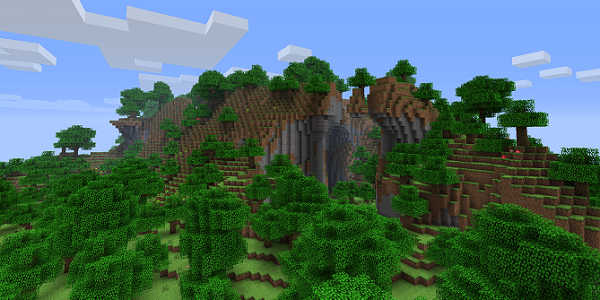
\includegraphics[width=7cm]{minecraft.png}
    \label{minecraft}
\end{figure}

La r�ponse � la question est la g�n�ration proc�durale. Cette technique a �t� beaucoup popularis� par un jeu vid�o indie nomm� Minecraft (voir figure~\ref{minecraft}). Par contre, il existe beaucoup de variantes � la g�n�ration proc�durale. L'article �tudi� se concentre sur la g�n�ration proc�durale de b�timents pour g�n�rer un environnement urbain r�aliste. Pour commencer, le fonctionnement de cette technique est d'utiliser des algorithme qui s'ex�cutent sur l'unit� de traitement d'un ordinateur pour g�n�rer un �l�ment. On ne sp�cifie pas directement le r�sultat de la g�n�ration ici parce qu'il est possible de g�n�rer pratiquement n'importe quel �l�ment gr�ce � cette technique. Elle offre aussi la possibilit� d'ajouter du hasard dans la g�n�ration pour ne pas obtenir toujours le m�me r�sutlat � chaque ex�cution. Elle est beaucoup utilis�e puisqu'il est possible d'ajouter de la vari�t� et de la rejouabilit� dans les jeux de nos jours. Par contre, au d�part, cette technique �tait beaucoup utilis�e pour �conomiser de l'espace lors de la cr�ation de jeux. Puisque certains �l�ments �taient g�n�r�s lorsque le jeu est en marche, il y avait moins de ressources � conserver en m�moire. Le premier exemple de g�n�ration proc�durale se trouve dans le jeu Akalabeth (1980) o� les cartes �taient g�n�r�es~\cite{AkalabethGen}. La g�n�ration proc�durale a beaucoup �t� popularis�e par l'arriv�e du jeu Minecraft. Certains jeux en font m�me un usage tr�s int�ressant. Par exemple, dans le jeu "Left 4 Dead", on g�n�re la difficult� de la mission courante d'apr�s les statistiques des joueurs ainsi que les �quipements qu'ils ont sur eux~\cite{Left4DeadAI}. On remarque donc que l'on peut g�n�rer n'importe quel �l�ment gr�ce � cette technique.

Avant l'�volution de la technique �labor�e dans l'article �tudi�, deux autres fa�on de g�n�rer des b�timents de fa�on proc�durale existaient.

\subsection{Premi�re Technique}
\label{ssect:first}
%%%%%%%%%%%%%%%%%%%%%%%%%%%%%%%%%%%%%%%%%%%%%%%%%%%%%%%%%%%%

Cette technique a �t� cr�e pour g�n�rer des grandes villes avec un minimum de donn�es statistiques et g�ographiques. Elle voulait aussi offrir un grand contr�le aux usagers~\cite{ParishMuller}. Cette technique se sert du principe des "L-system". Cette technique tient aussi compte de la cr�ation de routes pour connecter les diff�rents b�timents. Par ocntre, cette technique ajoute des d�tails sur les fa�ades des b�timents g�n�r�s � l'aide de nuanceurs. Ces chercheurs ont montr� une m�thode pour g�n�rer un grand environnements urbains compos�s d'un grand nombre de b�timents. Cependant, il y a un probl�me. Les d�tails que ajout�s aux fa�ades des b�timents peuvent causer des intersections dans les mod�les ce qui peut enlever l'effet de r�alisme recherch�.

\subsection{Deuxi�me Technique}
\label{ssect:second}
%%%%%%%%%%%%%%%%%%%%%%%%%%%%%%%%%%%%%%%%%%%%%%%%%%%%%%%%%%%%

Ici, les chercheurs ont voulu s'attaquer au probl�me de la g�n�ration de d�tails sur les fa�ade des b�timents g�n�r�s. Ils ont r�ussi � cr�er des d�tails qui sont en fait g�n�r�s � l'�tape g�om�trique. Ces d�tails sont donc compris dans le mod�le r�sultant et il n'est pas n�cessaire d'utiliser des nuanceurs pour ajouter du r�alisme aux fa�ades des b�timents. Par contre, avec cette technique, on s'attarde aux d�tails d'un seul b�timent � la fois. Il n'est donc pas possible de g�n�rer un grand environnement urbain comme dans la premi�re technique.

On remarque que l'on d�sire obtenir un m�lange de ces deux techniques. On d�sire un grand nombre de b�timents dans notre ville et que ces b�timents poss�dent des d�tails g�om�triques pour augmenter le r�alisme. Nous allons maintenant nous pencher sur la technique principale de l'article. On pr�cisera aussi en quoi cette m�thode est meilleure que les autres.

%%%%%%%%%%%%%%%%%%%%%%%%%%%%%%%%%%%%%%%%%%%%%%%%%%%%%%%%%%%%
\section{M�thode Choisie}
\label{sect:choisie}
%%%%%%%%%%%%%%%%%%%%%%%%%%%%%%%%%%%%%%%%%%%%%%%%%%%%%%%%%%%%

Intro to \sectref{choisie}.


\subsection{Th�orie}
\label{ssect:theorie}
%%%%%%%%%%%%%%%%%%%%%%%%%%%%%%%%%%%%%%%%%%%%%%%%%%%%%%%%%%%%

TH�ORIQUEMENT

\subsection{Exemples}
\label{ssect:ex}
%%%%%%%%%%%%%%%%%%%%%%%%%%%%%%%%%%%%%%%%%%%%%%%%%%%%%%%%%%%%

EXEMPLES

\subsection{Outil Existant}
\label{ssect:outil}
%%%%%%%%%%%%%%%%%%%%%%%%%%%%%%%%%%%%%%%%%%%%%%%%%%%%%%%%%%%%

OUTIL EXISTANT
%%%%%%%%%%%%%%%%%%%%%%%%%%%%%%%%%%%%%%%%%%%%%%%%%%%%%%%%%%%%
\section{Conclusion}
\label{sect:conclusion}
%%%%%%%%%%%%%%%%%%%%%%%%%%%%%%%%%%%%%%%%%%%%%%%%%%%%%%%%%%%%

Voil� une courte explication du fonctionnement de l'algorithme pr�sent� dans l'article �tudi�. L'algorithme offre des possibilit�s de g�n�ration infinie. La puissance de l'algorithme provient de la d�finition des r�gles. Comme prouv� dans l'exemple de la ville dans le style de Pompeii. Cette technique de g�n�ration a �t� d�velopp�e pour combiner les avantages de deux autres techniques qui ont �t� mises au point auparavant. De plus, il est facilement possible d'ajouter des �l�ments de hasard dans la g�n�ration. De cette fa�on, on peut cr�er plus d'une ville avec la m�me s�rie de r�gles.


\eject

\addcontentsline{toc}{section}{\refname}
\bibliography{biblio}

\end{document}
